\todo{to be weakened to the original version by endrullis}
\todo{maybe add the core lemma for estimating pushout object weight, but adapt to estimating DPO objects weight difference}
\begin{definition}[Decreasing Rules~\text{\cite[\textdef~5.9]{endrullis2024generalized}}]
    \label{def:decreasing_rule}
    Let $\mathcal{T} \mathop{=} (T,\mathbb{E},\mathcal{S}, w)$ be a finitary weighted type graph where $\mathcal{S}=\langle S, \mathop{\oplus}, \mathop{\odot}, 0, 1, \prec, \leq \rangle$ is a well-founded, commutative, \(\mathfrak{F}\) a DPO rewriting framework, $\rho \mathop{=} (L \overset{l}{\leftarrow} K \overset{r}{\rightarrow} R)$ a DPO rewriting rule. 

    \noindent
    The rule $\rho$ is \textbf{weakly decreasing} w.r.t. $\mathcal{T}$ in $\mathfrak{F}$ if 
            for every $t_K : K \mathop{\to} T$,
                $$ 
                  w_\mathcal{T}(\{l \mathop{\star} - \mathop{=} t_K\}) \mathop{\succeq} w_\mathcal{T}(\{r\star - \mathop{=} t_K\})$$
           
    \noindent
    The rule $\rho$ is \textbf{uniformly decreasing} w.r.t. $\mathcal{T}$ in $\mathfrak{F}$ if
        \begin{itemize}
            \item[]- there exists a context closure $c_\rho$ for $\rho$ and $\mathcal{T}$ in $\mathfrak{F}$, and
            \item[]- for every $t_K : K \mathop{\to} T$,
            \begin{itemize}
                \item[] $\bullet$ $\{l \mathop{\star} - \mathop{=} t_K\} \mathop{=} \emptyset \mathop{=} \{r \mathop{\star} - \mathop{=} t_K\}$, or
                \item[] $\bullet$ $w_\mathcal{T}(\{l \mathop{\star} - \mathop{=} t_K\}) \mathop{\succ}    w_\mathcal{T}(\{r \mathop{\star} - \mathop{=} t_K\})\mathop{+}\delta$.
            \end{itemize}
        \end{itemize}  
         
    \noindent
    The rule $\rho$ is
            \textbf{$\delta$-closure decreasing} w.r.t. $\mathcal{T}$ in $\mathfrak{F}$ if the following hold:
            \begin{itemize}
                \item[]- $S$ is strictly monotonic semiring,
                \item[]- $\rho$ is weakly decreasing,
                \item[]- there exists a context closure $c_\rho$ for $\rho$ and $\mathcal{T}$ in $\mathfrak{F}$,
                \item[]- $w_\mathcal{T}(\{l \mathop{\star} - \mathop{=} t_K\}) \mathop{\succ}  w_\mathcal{T}(\{r \mathop{\star} - \mathop{=} t_K\})$ for $t_K \mathop{=} l \mathop{\star} c_\rho$.
            \end{itemize}
\end{definition}

The following lemma states that decreasing rules reduce the weights of host graphs, provided specific constraints are satisfied.
\begin{lemma}[Decreasing steps~\text{\cite[Theorem C.3]{endrullis2024generalized}}]
    \label{lem:decreasing_step}
    \ \newline 
\begin{minipage}{0.7\textwidth}
    Let $\mathcal{T} \mathop{=} (T,\mathbb{E}, \mathcal{S}, w)$ be a finitary weighted type graph where $\mathcal{S} \mathop{=} \langle S, \mathop{\oplus}, \mathop{\odot}, 0, 1, \prec, \leq \rangle$ is a strong monotonic, commutative semiring, $\rho$ a rewriting rule and $\Delta \mathop{\in} \mathfrak{F}(\rho)$ a DPO diagram
    (shown on the right)   such that the following conditions hold:
\end{minipage}  
\begin{minipage}{0.3\textwidth}
    \begin{center}
        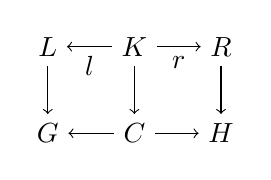
\begin{tikzpicture}[node distance=11mm]
          \node (I) {$K$};
          \node (L) [left of= I] {$L$};
          \node (R) [right of=I] {$R$}; 
          \node (G) [below of=L] {$G$};
          \node (C) [below of=I] {$C$};
          \node (H) [below of=R] {$H$};
        %   \node (T) [left=of $(L)!0.5!(G)$] {$T$};
        %   \draw [->] (L) to  node [label, above] {$c$}  (T);
        %   \draw [->] (G) to  node [label, below] {$\alpha$} (T);
          \draw [->] (I) to node [label, below] {$l$} (L);
          \draw [->] (I) to node [label, below] {$r$} (R);
          \draw [->] (L) to  (G);
          \draw [->] (I) to (C);
          \draw [->] (R) to (H);
          \draw [->] (C) to (G);
          \draw [->] (C) to (H);
        \end{tikzpicture}
      \end{center}
\end{minipage}
   \begin{itemize}
       \item $\operatorname{left}(\Delta)$ is weighable with \(\mathcal{T}\), and
       \item $\operatorname{right}(\Delta)$ is bounded above by \(\mathcal{T}\), and
       \item $w(e) \mathop{\succeq} 1_S$ for all $e \mathop{\in} \mathbb{E}$.
   \end{itemize}

   \noindent
  We have:
   \begin{itemize}
       \item $w_\mathcal{T}(G) \mathop{\succeq} w_\mathcal{T}(H)$ if $\rho$ is weakly decreasing,
       \item $w_\mathcal{T}(G) \mathop{\succ} w_\mathcal{T}(H)$ if $w(e) \mathop{\succeq} 1_S$ for all $e \mathop{\in} \mathbb{E}$, and $\rho$ is uniformly or closure decreasing.
   \end{itemize}
\end{lemma} 
\begin{proof}
   See the \hyperref[proof:decreasing_step]{Appendix}.
\end{proof}